\documentclass[tikz]{standalone}
\usepackage{amsmath} % for aligned
\usepackage{listofitems} % for \readlist to create arrays
\usetikzlibrary{arrows.meta} % for arrow size
\usepackage[outline]{contour} % glow around text
\contourlength{1.4pt}

% COLORS
\usepackage{xcolor}
\colorlet{myred}{red!80!black}
\colorlet{myblue}{blue!80!black}
\colorlet{mygreen}{green!60!black}
\colorlet{myorange}{orange!70!red!60!black}
\colorlet{mydarkred}{red!30!black}
\colorlet{mydarkblue}{blue!40!black}
\colorlet{mydarkgreen}{green!30!black}

% STYLES
\tikzset{
  >=latex, % for default LaTeX arrow head
  node/.style={thick,circle,draw=myblue,minimum size=22,inner sep=0.5,outer sep=0.6},
  node in/.style={node,green!20!black,draw=mygreen!30!black,fill=mygreen!25},
  node hidden/.style={node,blue!20!black,draw=myblue!30!black,fill=myblue!20},
  node convol/.style={node,orange!20!black,draw=myorange!30!black,fill=myorange!20},
  node out/.style={node,red!20!black,draw=myred!30!black,fill=myred!20},
  connect/.style={thick,mydarkblue}, %,line cap=round
  connect arrow/.style={-{Latex[length=4,width=3.5]},thick,mydarkblue,shorten <=0.5,shorten >=1},
  node 1/.style={node in}, % node styles, numbered for easy mapping with \nstyle
  node 2/.style={node hidden},
  node 3/.style={node out}
}
\def\nstyle{int(\lay<\Nnodlen?min(2,\lay):3)}

\begin{document}

% NEURAL NETWORK with coefficients, uniform arrows
\newcommand\setAngles[3]{
  \pgfmathanglebetweenpoints{\pgfpointanchor{#2}{center}}{\pgfpointanchor{#1}{center}}
  \pgfmathsetmacro\angmin{\pgfmathresult}
  \pgfmathanglebetweenpoints{\pgfpointanchor{#2}{center}}{\pgfpointanchor{#3}{center}}
  \pgfmathsetmacro\angmax{\pgfmathresult}
  \pgfmathsetmacro\dang{\angmax-\angmin}
  \pgfmathsetmacro\dang{\dang<0?\dang+360:\dang}
}

% NEURAL NETWORK with coefficients, shifted
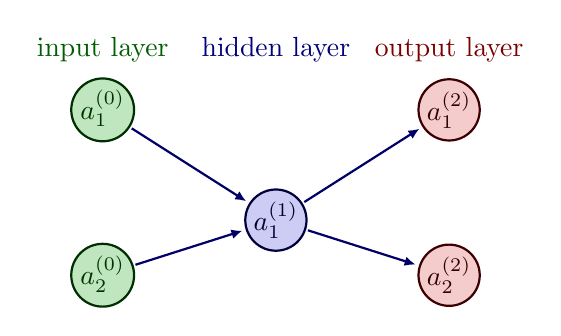
\begin{tikzpicture}[x=2.2cm,y=1.4cm]
  \message{^^JNeural network, shifted}
  \readlist\Nnod{2,1,2} % array of number of nodes per layer
  \readlist\Nstr{2,1,2} % array of string number of nodes per layer
  \readlist\Cstr{\strut a^{(0)},a^{(\prev)},a^{(\prev)}} % array of coefficient symbol per layer
  \def\yshift{0.5} % shift last node for dots
  
  \message{^^J  Layer}
  \foreachitem \N \in \Nnod{ % loop over layers
    \def\lay{\Ncnt} % alias of index of current layer
    \pgfmathsetmacro\prev{int(\Ncnt-1)} % number of previous layer
    \message{\lay,}
    \foreach \i [evaluate={\c=int(\i==\N); \y=\N/2-\i-\c*\yshift;
                 \index=(\i<\N?int(\i):"\Nstr[\lay]");
                 \a=\lay; \n=\nstyle;}] in {1,...,\N}{ % loop over nodes
      % NODES
      \node[node \n] (N\lay-\i) at (\a,\y) {$\Cstr[\lay]_{\index}$};
      % \node[node \nstyle] (N\lay-\i) at (\lay,\N/2-\i+0.5*\N) {$\Cstr[\lay]_{\i}$};
      
      % CONNECTIONS
      \ifnum\lay>1 % connect to previous layer
        \foreach \j in {1,...,\Nnod[\prev]}{ % loop over nodes in previous layer
          \draw[connect arrow] (N\prev-\j) -- (N\lay-\i);
          % node[weight label] {0.5};
        }
      \fi % else: nothing to connect first layer
      
    }
    % \path (N\lay-\N) --++ (0,1+\yshift) node[midway,scale=1.5] {$\vdots$};
  }
  
  % LABELS
  \node[above=2,align=center,mygreen!60!black] at (N1-1.90) {input layer};
  \node[above=42,align=center,myblue!60!black] at (N2-1.90) {hidden layer};
  \node[above=2,align=center,myred!60!black] at (N3-1.90) {output layer};
  
\end{tikzpicture}

\end{document}